%% 1
%TODO We solved for...
In this exercise we begin by solving Laplace's equation $\nabla^2 \phi(\mathbf{r}) = 0$ numerically in the square $-1\le x \le 1$ and $-1\le y \le 1$ with grid size $h=0.1$.
We are going to use the relaxational method to solve this and to start the iteration off we initialize $\phi$
to $0.1$ except at the origin and boundaries where a constant value is imposed, $\phi(1,y) = \phi(-1,y) = \phi(x,1) = \phi(x,-1) = 0$ and $\phi(0,0) = -1$
The result for iteration 100 and 1000 can be seen in table \ref{table:exc1_laplace}.
\begin{table}[h!]
\caption{Values of $\phi$ at $y=0$ for different iterations.}
\center
\begin{tabular}{|c|c|c|}
\hline 
iteration & 100 & 1000 \\ 
\hline 
x=0 & -1.0000 & -1.0000 \\ 
\hline 
x=0.1 & -0.5668 & -0.6067 \\ 
\hline 
x=0.2 & -0.3729 & -0.4284 \\ 
\hline 
x=0.3 & -0.2605 &  -0.3230 \\ 
\hline 
x=0.4 & -0.1871 & -0.2492 \\ 
\hline 
x=0.5 & -0.1332 & -0.1921 \\ 
\hline 
x=0.6 & -0.0941 & -0.1449 \\ 
\hline 
x=0.7 & -0.0630 & -0.1040 \\ 
\hline 
x=0.8 &  -0.0391 & -0.0673 \\ 
\hline 
x=0.9 & -0.0184 & -0.0331 \\ 
\hline 
x=1 & 0 & 0 \\ 
\hline 
\end{tabular}
\label{table:exc1_laplace}
\end{table}
\FloatBarrier

As can be seen in table \ref{table:exc1_laplace} the values at different points vary by almost a factor of two at some points. So I decided to stop iterating when the \emph{relative error}---defined as the 2-norm of the difference between the vector $\phi$ and it's previous values, divided by the absolute maximum value of $phi$---is less than a \emph{relative tolerance} that is much less than unity. In our case, $relative tolerance = 1e-6$.
The results can be seen in fig. \ref{fig:exc1_laplace}.
 
%% 2
\begin{figure}[h!]
	\centering
	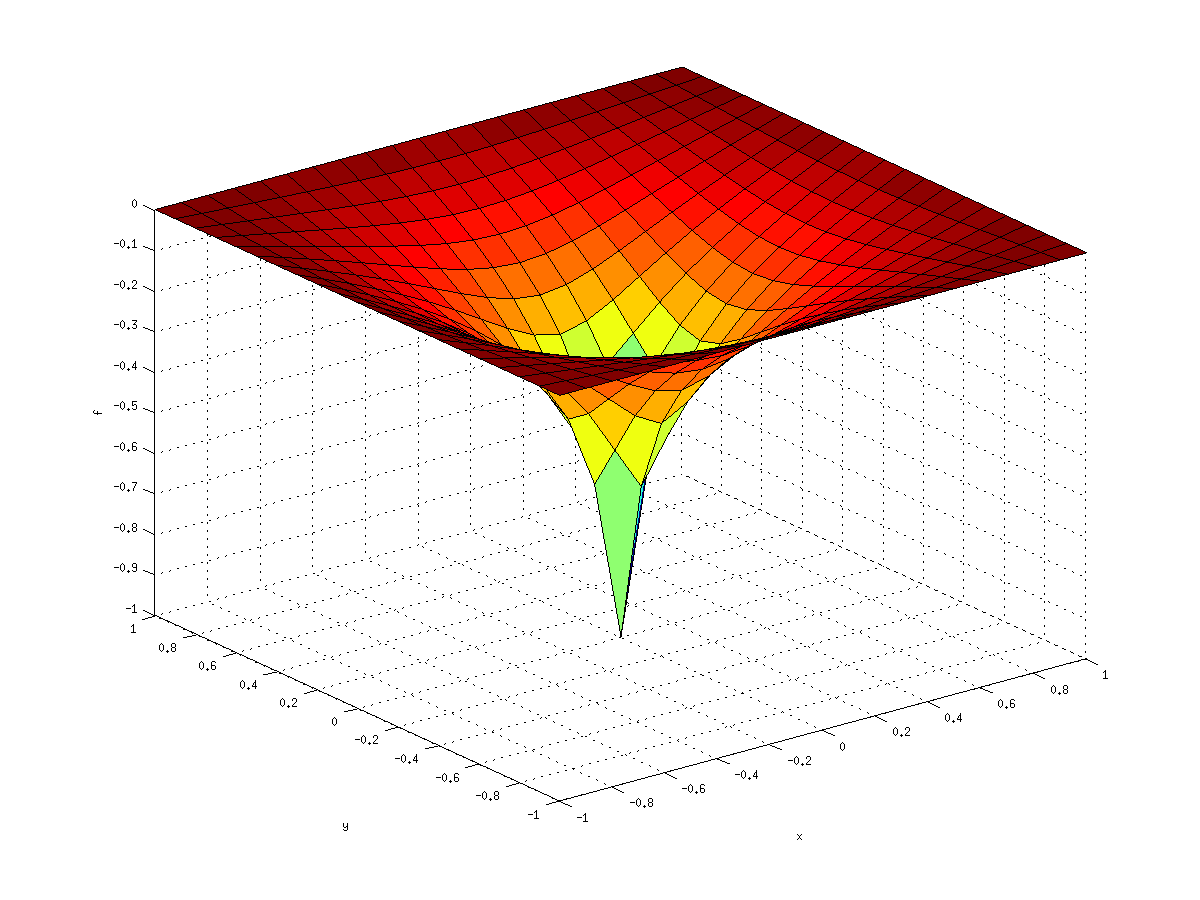
\includegraphics[width=0.8\textwidth]{img/exc1_laplace}
	\caption{$\phi(x,y)$ after 1931 iterations.}
	\label{fig:exc1_laplace}
\end{figure}

%% 3
The electric field is defined as $\mathbf{E}(x,y) = -\nabla \phi(x,y)$. I calculated this for the line 
$y=0 and 0.1 \le x \le 0.9$ with the results in fig. \ref{fig:exc1_E}. The loglog plot in fig. \ref{fig:exc1_logE} could show that 
$log(|\mathbf{E}|) \propto log(1/x)$ which would mean that $|\mathbf{E}| \propto \ 1/x$ on this line.
Deriving $\mathbf{E}$ analytically we get
\[
\nabla^2 \phi = 0 \implies \nabla \cdot \mathbf{E} = 0
\]
assuming radial symmetry, so that $\mathbf{E} = E \hat{r}$ we get
\[
\frac{1}{r} \frac{\partial}{\partial r} \left( E + r \frac{\partial E}{\partial r} \right)
\iff r \frac{\partial E}{\partial r} + E = 0 \qquad for \; r \neq 0.
\]
The solution for this is 
\begin{equation}
E = a r^{-1}, \; a=constant, \qquad r \neq 0
\end{equation}
and for the line that was plotted in fig. \ref{fig:exc1_logE} this is equivalent to $E \propto 1/x$ and so the analytical
solution agrees with the numerical solution.
\begin{figure}[h!]
	\centering
	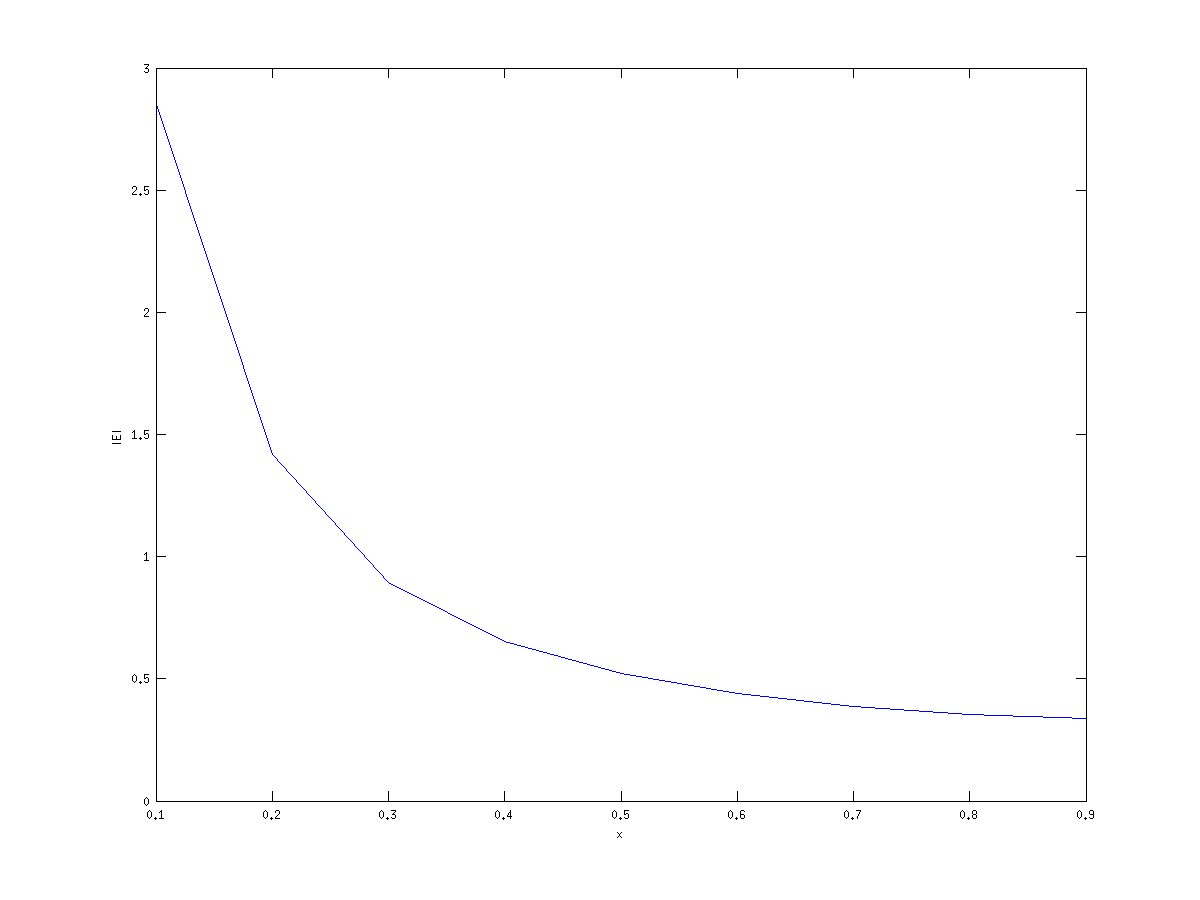
\includegraphics[width=0.8\textwidth]{img/exc1_E}
	\caption{$\phi(x,y)$ after 1931 iterations.}
	\label{fig:exc1_E}
\end{figure}
\begin{figure}[h!]
	\centering
	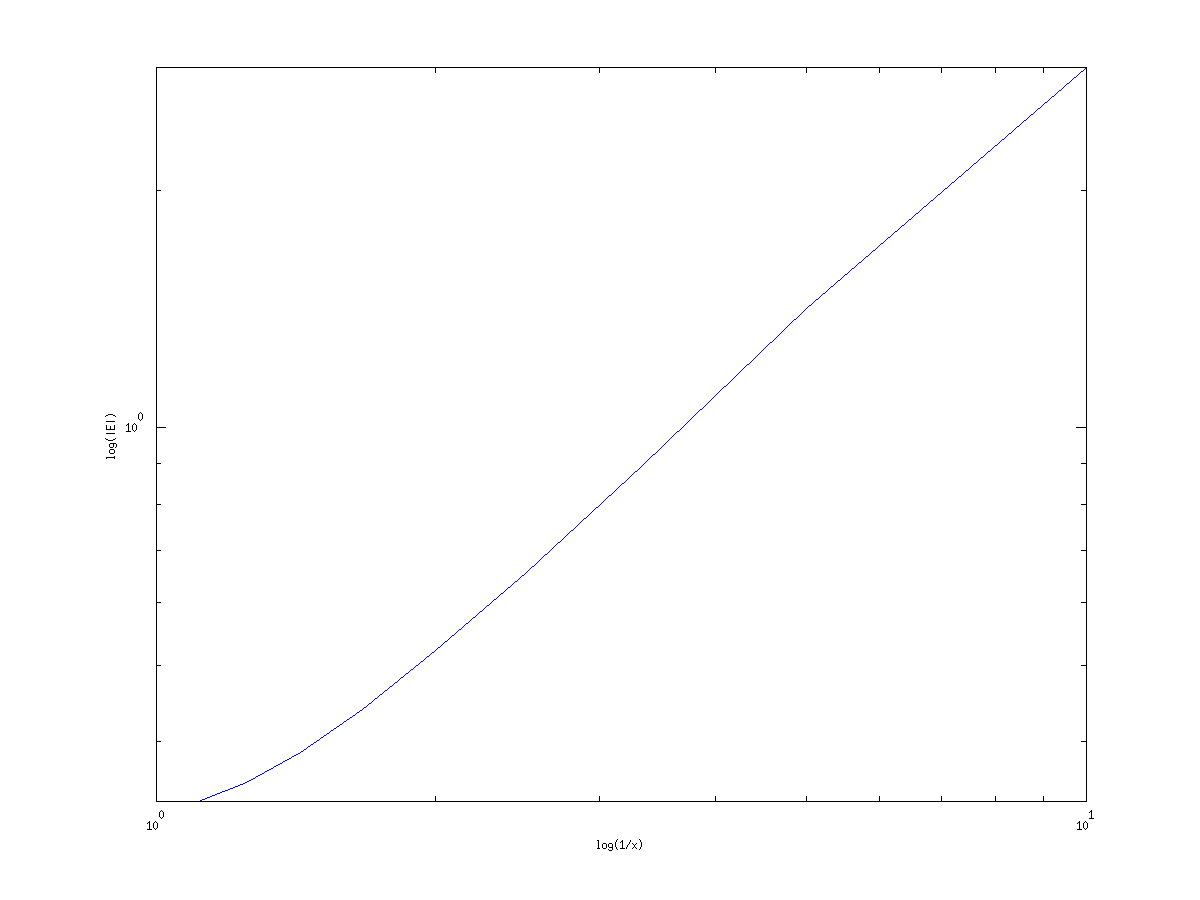
\includegraphics[width=0.8\textwidth]{img/exc1_logE}
	\caption{$\phi(x,y)$ after 1931 iterations.}
	\label{fig:exc1_logE}
\end{figure}

\FloatBarrier
In general the Laplace equation can be extended to Poisson's equation
\begin{equation}
\nabla^2\phi(\mathbf{r}) = -4\pi \rho(\mathbf{r}).
\label{eq:exc1_poisson}
\end{equation}
To solve this numerically we make it discrete; the laplacian can be written as
\[
\nabla^2 \phi(x,y) \approx \frac{\phi(x+h,y)+\phi(x-h,y)-2\phi(x,y)}{h^2} + \frac{\phi(x,y+h)+\phi(x,y-h)-2\phi(x,y)}{h^2}
\]
and so we get
\[
\frac{\phi(x+h,y)+\phi(x-h,y)-2\phi(x,y)}{h^2} + \frac{\phi(x,y+h)+\phi(x,y-h)-2\phi(x,y)}{h^2} = -4 \pi \rho(x,y)
\]
which can be solved for $\phi(x,y)$. Using the relaxational method to iteratively get the function $\phi(x,y)$ we get the updating scheme
\begin{equation}
\phi_{n+1}(x,y) = \frac{\phi_n(x+h,y)+\phi_n(x-h,y)+\phi_n(x,y+h)}{4} + \pi h^2 \rho(x,y).
\end{equation}

I solved this for $\rho(x,y) = 1/h^2 \delta_{x,0}\delta_{0,y}$ and the results can be seen in fig. \ref{fig:exc1_poisson}
\begin{figure}[h!]
	\centering
	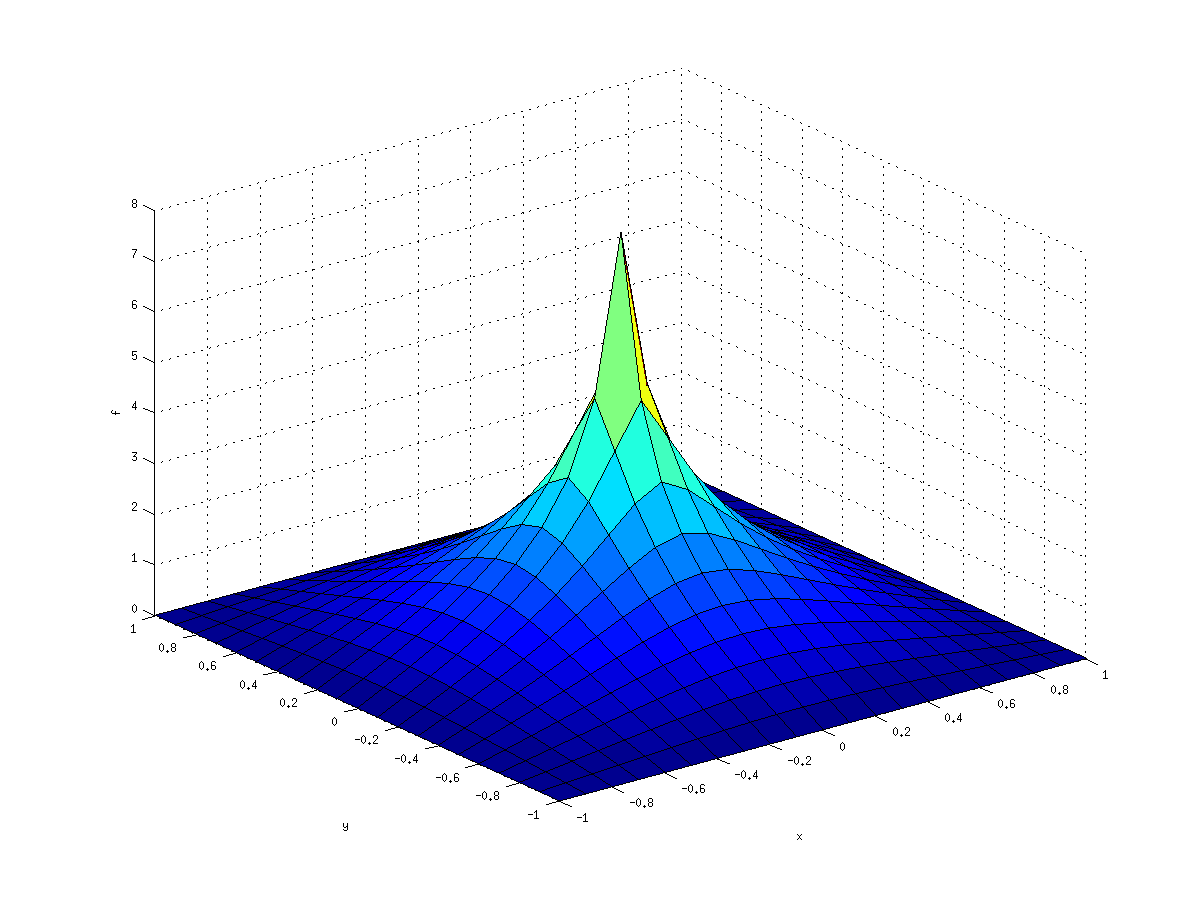
\includegraphics[width=0.8\textwidth]{img/exc1_poisson}
	\caption{$\phi(x,y)$ after 1931 iterations.}
	\label{fig:exc1_poisson}
\end{figure}